\chapter{Das Dirac-Meer, Fermionenmassen und Vierkomponentenspinoren}

\section{Rechtslaufende Fermionen und das Dirac-Meer}

Die Dirac-Gleichung ist eine Gleichung für Fermionen. Relativistische Bosonen erfüllen andere Gleichungen, etwa die Klein--Gordon-Gleichung oder die Maxwell-Gleichungen. Das einfachste Beispiel gilt in einer Raumdimension und beschreibt zunächst Teilchen und Antiteilchen, die sich nur nach rechts bewegen können.

Wir beginnen mit einer ebenen Welle,
\begin{equation}
\psi(x,t)=\psi_0 e^{i(kx-\omega t)}.
\end{equation}
Ihre Phasengeschwindigkeit ist
\begin{equation}
v_{\mathrm{ph}}=\frac{\omega}{k}.
\end{equation}
Die Vorzeichen von \(k\) und \(\omega\) sind entscheidend. Haben sie dasselbe Vorzeichen, bewegt sich die Phase nach rechts; haben sie entgegengesetzte Vorzeichen, bewegt sie sich nach links. Wenn \(\omega\) proportional zu \(k\) ist, stimmen Phasen- und Gruppengeschwindigkeit überein:
\begin{equation}
v_{\mathrm{g}}=\frac{d\omega}{dk}=\frac{\omega}{k}.
\end{equation}

Betrachten wir die Differentialgleichung erster Ordnung
\begin{equation}
\frac{\partial\psi}{\partial x}
+
\frac{\partial\psi}{\partial t}
=0.
\end{equation}
Setzt man die ebene Welle ein, erhält man
\begin{equation}
ik\psi-i\omega\psi=0,
\end{equation}
und damit
\begin{equation}
\omega=k.
\end{equation}
Die Welle bewegt sich also nach rechts. Entsprechend bezeichnen wir das Feld mit
\begin{equation}
\frac{\partial\psi_R}{\partial t}
=
-\frac{\partial\psi_R}{\partial x}.
\end{equation}

Mit wiederhergestellter Lichtgeschwindigkeit lautet die Gleichung in dimensionsbehafteter Form
\begin{equation}
\frac{\partial\psi_R}{\partial x}
+
\frac{1}{c}\frac{\partial\psi_R}{\partial t}
=0,
\end{equation}
also
\begin{equation}
\omega=ck.
\end{equation}
Von nun an gilt \(c=1\). Bei \(\hbar=1\) ist \(\omega\) zugleich die Energie eines Quants.

\begin{figure}[htbp]
\centering
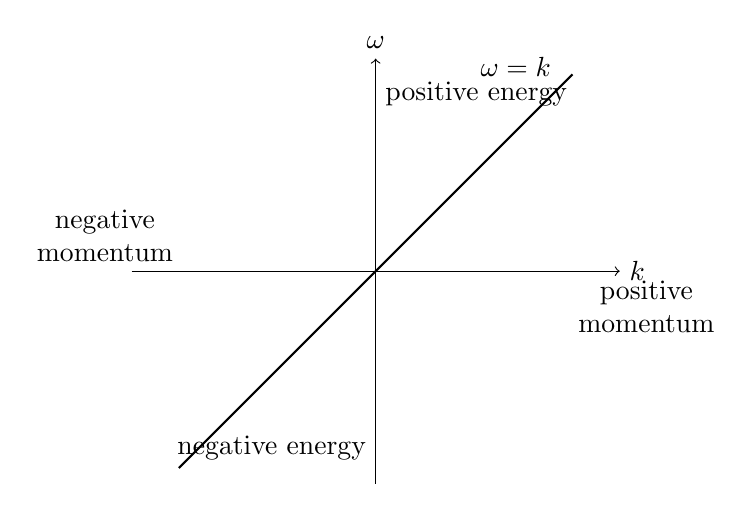
\begin{tikzpicture}[scale=1.0]
\draw[->] (-3.1,0) -- (3.1,0) node[right] {$k$};
\draw[->] (0,-2.7) -- (0,2.7) node[above] {$\omega$};
\draw[thick] (-2.5,-2.5) -- (2.5,2.5);
\node[above left] at (2.35,2.35) {$\omega=k$};
\node[below right,align=center] at (2.45,0) {positive\\momentum};
\node[above left,align=center] at (-2.45,0) {negative\\momentum};
\node[right] at (0,2.25) {positive energy};
\node[left] at (0,-2.25) {negative energy};
\end{tikzpicture}
\caption{Die masselose Dispersionsrelation für rechtslaufende Wellen \(\omega=k\) besitzt positive und negative Energiezweige.}
\end{figure}

Die Gerade hat eine schwerwiegende Konsequenz. Für positive Werte von \(k\) ist die Energie positiv, für negative Werte von \(k\) ist sie negativ. Dennoch beschreiben beide Bereiche rechtslaufende Wellen, denn \(\omega/k=1\) gilt auf der gesamten Geraden.

Ein Elektron auf dem positiven Energiezweig könnte in einen niedrigeren Zustand fallen, ein Photon positiver Energie emittieren, erneut fallen und so das Energiespektrum immer weiter hinabsteigen: eine Stufe nach der anderen. Kein Elektron wäre stabil. Schwerwiegender noch: Die Welt würde ihre Energie verringern, indem sie immer mehr Elektronen negativer Energie erzeugt.

Das Pauli-Ausschlussprinzip für Fermionen liefert die Lösung. Wir besetzen alle Elektronenzustände negativer Energie. In einen bereits besetzten Zustand kann kein weiteres Elektron eintreten, sodass der vollständig besetzte Bereich negativer Energien einen unbegrenzten Abstieg verhindert. Dieser gefüllte Bereich heißt Dirac-Meer; sein vollständig besetzter Zustand ist der Grundzustand oder das Vakuum.

\begin{classroomqa}
\lecturetimestamp{00:07:19}
\audiencequestion{Gibt es unendlich viele tiefere Zustände negativer Energie?}
\lecturerresponse{Ja. Bei diskreten Impulsen ähnelt das Spektrum einer unendlichen Treppe, bei kontinuierlichen Impulsen einem durchgehenden Abhang. Das Auffüllen des Dirac-Meers verhindert, dass ein Elektron unbegrenzt weiter absteigt. Ein Übergang zu einem tieferen Zustand mit Emission eines Photons kann jedoch weiterhin möglich sein, sofern ein solcher Zustand unbesetzt ist.}
\end{classroomqa}

Das erklärt, warum eine Gleichung mit diesem Spektrum als fermionische Theorie quantisiert werden muss. Wären die Quanten Bosonen, könnten beliebig viele von ihnen denselben tieferen Zustand besetzen. Das Auffüllen des Bereichs negativer Energien würde das Vakuum dann nicht stabilisieren.

Das Bild des gefüllten Meers führt auch zu Antiteilchen. Im Vakuum sind alle Niveaus negativer Energie besetzt und alle Niveaus positiver Energie leer. Ein Elektron kann aus einem beliebigen besetzten Niveau negativer Energie in ein beliebiges unbesetztes Niveau positiver Energie gehoben werden; die Anfangs- und Endniveaus müssen nicht symmetrisch liegen.

\begin{figure}[htbp]
\centering
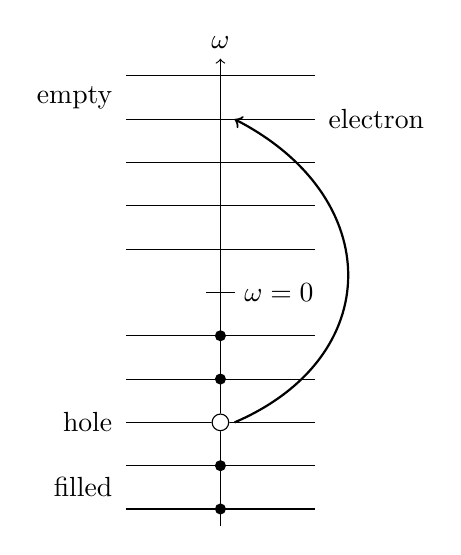
\begin{tikzpicture}[x=1cm,y=0.55cm]
\draw[->] (0,-5.4) -- (0,5.4) node[above] {$\omega$};
\draw (-0.18,0) -- (0.18,0) node[right] {$\omega=0$};
\foreach \y in {-5,-4,-3,-2,-1} {
  \draw (-1.2,\y) -- (1.2,\y);
  \fill (0,\y) circle (2pt);
}
\foreach \y in {1,2,3,4,5} {
  \draw (-1.2,\y) -- (1.2,\y);
}
\draw[->,thick] (0.18,-3) .. controls (2.1,-1.5) and (2.1,2.2) .. (0.18,4);
\draw[white,fill=white] (0,-3) circle (3pt);
\draw (0,-3) circle (3pt);
\node[left] at (-1.25,-3) {hole};
\node[left] at (-1.25,-4.5) {filled};
\node[left] at (-1.25,4.5) {empty};
\node[right] at (1.25,4) {electron};
\end{tikzpicture}
\caption{Wird ein Elektron aus einem besetzten Zustand negativer Energie angehoben, entsteht ein Elektron positiver Energie, und im gefüllten Meer bleibt ein Loch zurück.}
\end{figure}

Entfernt man ein Elektron negativer Energie, steigt die Energie gegenüber dem Vakuum; das Loch hat daher positive Energie. Auf dem Zweig \(\omega=k\) hatte auch das entfernte Elektron negativen Impuls. Durch das Entfernen eines negativen Impulses bleibt ein positiver Impulsüberschuss zurück; das Loch hat also positiven Impuls. Wenn die Ladung des Elektrons als negativ angesetzt wird, hat das fehlende Elektron positive Ladung. Das Loch ist somit ein Antiteilchen mit positiver Energie und positivem Impuls, während das angeregte Elektron negative Ladung, positive Energie und positiven Impuls hat. Jede reale Anregung in dieser Theorie mit nur einem Zweig bewegt sich nach rechts.

Das Feld \(\psi_R\) wird aus fermionischen Erzeugungs- und Vernichtungsoperatoren aufgebaut. Die Deutung als Teilchen und Loch betrifft daher die vom Feld erzeugten und entfernten Quanten, nicht nur eine klassische Welle.

Eine Asymmetrie bleibt bestehen. Das Meer rechtslaufender Zustände enthält Zustände negativer Energie mit negativem Impuls. Sein formaler Gesamtimpuls ist enorm und nach links gerichtet. Man kann den Vakuumimpuls durch Abziehen dieser Konstanten gleich null setzen; strukturell bleibt der Zustand jedoch unausgewogen: Teilchen und Antiteilchen bewegen sich nur nach rechts, während das gefüllte Vakuum aus Zuständen mit negativem Impuls besteht.

\section{Der linkslaufende Zweig und ein ausgeglichenes Vakuum}

Für ein Gleichgewicht zwischen links und rechts braucht man ein zweites, unabhängiges Feld mit eigenen Erzeugungs- und Vernichtungsoperatoren. Es erfülle
\begin{equation}
\frac{\partial\psi_L}{\partial t}
=
+\frac{\partial\psi_L}{\partial x}.
\end{equation}
Für denselben Ansatz einer ebenen Welle gilt
\begin{equation}
-i\omega\psi_L=ik\psi_L,
\end{equation}
also
\begin{equation}
\omega=-k.
\end{equation}
Diese zweite Gerade ist das Spiegelbild von \(\omega=k\). Ihr positiver Energiezweig beschreibt linkslaufende Teilchen; auch ihr negativer Energiezweig muss aufgefüllt werden.

\begin{figure}[htbp]
\centering
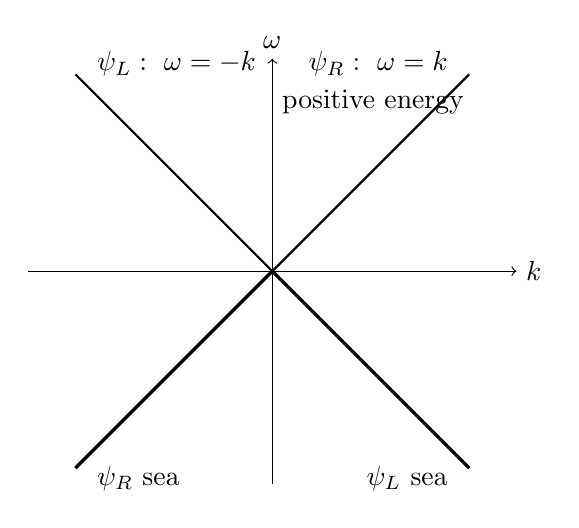
\begin{tikzpicture}[scale=1.0]
\draw[->] (-3.1,0) -- (3.1,0) node[right] {$k$};
\draw[->] (0,-2.7) -- (0,2.7) node[above] {$\omega$};
\draw[thick] (-2.5,-2.5) -- (2.5,2.5);
\draw[thick] (-2.5,2.5) -- (2.5,-2.5);
\draw[very thick] (-2.5,-2.5) -- (0,0);
\draw[very thick] (0,0) -- (2.5,-2.5);
\node[above left] at (2.35,2.35) {$\psi_R:\ \omega=k$};
\node[above right] at (-2.35,2.35) {$\psi_L:\ \omega=-k$};
\node[right] at (0,2.15) {positive energy};
\node[below right] at (-2.35,-2.35) {$\psi_R$ sea};
\node[below left] at (2.35,-2.35) {$\psi_L$ sea};
\end{tikzpicture}
\caption{Unabhängige rechts- und linkslaufende Felder ergeben gespiegelte masselose Zweige; im Vakuum sind die beiden Halbzweige negativer Energie aufgefüllt.}
\end{figure}

Nachdem beide Meere negativer Energie aufgefüllt sind, gibt es gleich viele besetzte Zustände für linkslaufende wie für rechtslaufende Wellen. Ihre Vakuumimpulse gleichen sich aus. Teilchen- und Lochanregungen können sich nun in beide Richtungen bewegen.

\begin{classroomqa}
\lecturetimestamp{00:15:58}
\audiencequestion{Lässt sich das Problem negativer Energien behandeln, ohne gefüllte Zustände und Löcher zu postulieren?}
\lecturerresponse{Dieselbe Theorie lässt sich auch anders beschriften. Einen besetzten Zustand eines Elektrons negativer Energie kann man als leeren Zustand eines Antiteilchens bezeichnen; dann umfasst die physikalische Beschreibung nur Teilchen und Antiteilchen positiver Energie. Das Bild des gefüllten Meers bleibt eine nützliche Konsistenzprüfung, ähnlich einem gefüllten Band in einem Metall: Entfernt man ein Elektron, entsteht ein Loch, während eine Anregung sowohl ein Teilchen als auch ein Loch hervorbringt.}
\end{classroomqa}

Die bisher betrachteten Anregungen sind masselos. Ihre Dispersionsrelationen sind linear und ihre Geschwindigkeiten haben den Betrag \(1\); sie bewegen sich also mit Lichtgeschwindigkeit. Als Nächstes stellt sich die Frage, wie man ihnen eine Masse geben kann.

\section{Zwei Komponenten und der Massenterm}

Zunächst fassen wir die beiden Felder zu einer Spalte zusammen:
\begin{equation}
\Psi=
\begin{pmatrix}
\psi_R\\
\psi_L
\end{pmatrix}.
\end{equation}
Das ist zunächst lediglich eine kompakte Schreibweise für zwei unabhängige Gleichungen. Definieren wir
\begin{equation}
\alpha=
\begin{pmatrix}
1&0\\
0&-1
\end{pmatrix}.
\end{equation}
Dann lauten die Gleichungen für rechts- und linkslaufende Wellen
\begin{equation}
\frac{\partial\Psi}{\partial t}
=
-\alpha\frac{\partial\Psi}{\partial x}.
\end{equation}

\begin{figure}[htbp]
\centering
\includegraphics[width=0.78\textwidth]{lecture_06_figure_02.png}
\caption{Die Felder \(\psi_R\) und \(\psi_L\) bilden einen zweikomponentigen Spinor; \(\alpha\) unterscheidet die beiden masselosen Zweige.}
\lectureframe{00:20:36}
\end{figure}

Auf eine ebene Welle angewandt liefern die Operatoren
\begin{equation}
i\partial_t
\quad\hbox{and}\quad
-i\partial_x
\end{equation}
der Reihe nach \(\omega\) und \(k\). Daher lässt sich die Matrixgleichung abkürzend schreiben als
\begin{equation}
\omega=\alpha k.
\end{equation}
Für die obere Komponente bedeutet dies \(\omega=k\), für die untere \(\omega=-k\). Die Schreibweise fasst die beiden Gleichungen zusammen, führt aber keine neue Physik ein.

Elektronen sind nicht masselos und bewegen sich nicht mit Lichtgeschwindigkeit. Eine naheliegende Formel für ihre Energie ist die nichtrelativistische kinetische Energie \(k^2/(2m)\). Sie kann hier jedoch nicht als Ausgangspunkt dienen: Der masselose Grenzfall betrifft bereits Bewegungen mit Lichtgeschwindigkeit. Die relativistische Beziehung lautet
\begin{equation}
\omega^2=k^2+m^2,
\end{equation}
oder, wenn man beide Energiezweige berücksichtigt,
\begin{equation}
\omega=\pm\sqrt{k^2+m^2}.
\end{equation}
Für \(m=0\) erhält man daraus \(\omega=k\) und \(\omega=-k\).

\begin{classroomqa}
\lecturetimestamp{00:25:23}
\audiencequestion{Werden hier Einheiten mit \(c=1\) verwendet, und wie erhält man die Geschwindigkeit eines massiven Teilchens?}
\lecturerresponse{Ja. Die Geschwindigkeit eines Wellenpakets ist die Gruppengeschwindigkeit; auf dem positiven Energiezweig gilt \(v_{\mathrm g}=d\omega/dk=k/\sqrt{k^2+m^2}\). Die Dispersionsrelation selbst enthält somit bereits die Verringerung der Geschwindigkeit eines massiven Teilchens gegenüber \(c=1\).}
\end{classroomqa}

\begin{classroomqa}
\lecturetimestamp{00:26:29}
\audiencequestion{Ist \(\omega\) in der Kurzschreibweise \(\omega=\alpha k\) ein Vektor oder eine Matrix?}
\lecturerresponse{Die Kurzschreibweise steht für eine Operatorgleichung, die auf die zweikomponentige Wellenfunktion wirkt. Hier bedeutet \(\omega\) \(i\partial_t\), \(k\) bedeutet \(-i\partial_x\), und \(\alpha\) ist die Matrix, die auf den Komponentenindex wirkt. Die skalaren Größen \(\omega\) und \(k\) nehmen erst auf einer ebenen Welle ihre numerischen Eigenwerte an.}
\end{classroomqa}

Wir behalten die Gleichung erster Ordnung bei und versuchen die einfachste massenabhängige Erweiterung:
\begin{equation}
\omega=\alpha k+\beta m.
\end{equation}
Das Objekt \(\beta\) muss eine Matrix sein, da es auf dasselbe zweikomponentige Feld wirkt wie \(\alpha\). Seine Algebra ergibt sich durch Quadrieren:
\begin{align}
\omega^2
&=(\alpha k+\beta m)(\alpha k+\beta m)\\
&=\alpha^2k^2+\beta^2m^2
+\alpha\beta\,km+\beta\alpha\,mk\\
&=\alpha^2k^2+\beta^2m^2
+(\alpha\beta+\beta\alpha)km.
\end{align}
Damit für alle \(k\) und \(m\) \(k^2+m^2\) gilt, muss
\begin{equation}
\alpha^2=I,
\qquad
\beta^2=I,
\qquad
\alpha\beta+\beta\alpha=0.
\end{equation}

Zwei gewöhnliche, von null verschiedene Zahlen können die letzte Bedingung nicht erfüllen: Für Zahlen ergäbe sich \(2\alpha\beta=0\), im Widerspruch dazu, dass beide Quadrate \(1\) sein sollen. Matrizen können antikommutieren. Insbesondere kann \(\beta\) nicht gleich \(\alpha\) sein, denn dann wäre
\begin{equation}
\alpha\beta+\beta\alpha=2\alpha^2=2I.
\end{equation}

Wir wählen
\begin{equation}
\beta=
\begin{pmatrix}
0&1\\
1&0
\end{pmatrix}.
\end{equation}
Das Quadrat lässt sich Eintrag für Eintrag überprüfen:
\begin{equation}
\begin{aligned}
\beta^2
&=
\begin{pmatrix}
0&1\\
1&0
\end{pmatrix}
\begin{pmatrix}
0&1\\
1&0
\end{pmatrix}\\
&=
\begin{pmatrix}
0\cdot0+1\cdot1&0\cdot1+1\cdot0\\
1\cdot0+0\cdot1&1\cdot1+0\cdot0
\end{pmatrix}
=
\begin{pmatrix}
1&0\\
0&1
\end{pmatrix}.
\end{aligned}
\end{equation}
Die Reihenfolge der Multiplikation ist entscheidend:
\begin{align}
\alpha\beta
&=
\begin{pmatrix}
1&0\\
0&-1
\end{pmatrix}
\begin{pmatrix}
0&1\\
1&0
\end{pmatrix}
=
\begin{pmatrix}
0&1\\
-1&0
\end{pmatrix},\\
\beta\alpha
&=
\begin{pmatrix}
0&1\\
1&0
\end{pmatrix}
\begin{pmatrix}
1&0\\
0&-1
\end{pmatrix}
=
\begin{pmatrix}
0&-1\\
1&0
\end{pmatrix}.
\end{align}
Also gilt
\begin{equation}
\alpha\beta=-\beta\alpha,
\qquad
\alpha\beta+\beta\alpha=0.
\end{equation}
Es gibt auch andere äquivalente Matrizenwahlmöglichkeiten; mit dieser werden die Komponentengleichungen jedoch besonders anschaulich.

Mit den Differentialoperatoren wieder eingesetzt ergibt sich die massive Gleichung
\begin{equation}
i\frac{\partial\Psi}{\partial t}
=
-i\alpha\frac{\partial\Psi}{\partial x}
+m\beta\Psi.
\end{equation}
Die Matrix \(\beta\) vertauscht die beiden Komponenten:
\begin{equation}
\beta
\begin{pmatrix}
\psi_R\\
\psi_L
\end{pmatrix}
=
\begin{pmatrix}
\psi_L\\
\psi_R
\end{pmatrix}.
\end{equation}
Folglich gilt
\begin{align}
i\dot{\psi}_R
&=-i\frac{\partial\psi_R}{\partial x}+m\psi_L,\\
i\dot{\psi}_L
&=+i\frac{\partial\psi_L}{\partial x}+m\psi_R.
\end{align}

Der Massenterm koppelt Felder, die in der masselosen Theorie unabhängig waren. Die Gleichung für die obere Komponente enthält die untere Komponente, und die Gleichung für die untere enthält die obere. Diese Kopplung ist es, was eine Dirac-Masse ausmacht. Die Gleichungen sind translationsinvariant und erhalten daher den Impuls; die Masse ihrer Teilchenanregungen ist \(m\).

\begin{classroomqa}
\lecturetimestamp{00:38:25}
\audiencequestion{Ist eine Lösung automatisch Lorentz-invariant?}
\lecturerresponse{Eine bestimmte Lösung sollte unter einer Lorentz-Transformation nicht unverändert bleiben. Ein Zustand mit einem bestimmten Impuls wird in einen Zustand mit dem transformierten Impuls überführt. Die passende Aussage ist daher Kovarianz. Die Beziehung \(\omega^2=k^2+m^2\) ist eine wichtige Lorentz-invariante Prüfung; volle Kovarianz verlangt jedoch auch das Transformationsgesetz des Spinors \(\Psi\), das noch nicht hergeleitet wurde.}
\end{classroomqa}

\section{Das Ruhesystem und die Bedeutung der Komponenten}

Ein masseloses Teilchen lässt sich nicht in Ruhe versetzen, ein massives hingegen schon. Im Ruhezustand gilt \(k=0\), sodass die Wellenfunktion keine Ortsabhängigkeit hat und
\begin{equation}
\omega=\beta m.
\end{equation}
Die Differentialgleichung vereinfacht sich zu
\begin{equation}
i\frac{d\Psi}{dt}=m\beta\Psi.
\end{equation}
In Komponenten lautet sie
\begin{align}
i\dot{\psi}_R&=m\psi_L,\\
i\dot{\psi}_L&=m\psi_R.
\end{align}
Beide Nebendiagonaleinträge von \(\beta\) sind \(+1\); in keiner dieser Gleichungen tritt daher ein zusätzliches Minuszeichen auf.

Durch Addition und Subtraktion der Komponenten entkoppeln sich die Gleichungen. Wir definieren
\begin{equation}
\psi_+=\psi_R+\psi_L,
\qquad
\psi_-=\psi_R-\psi_L.
\end{equation}
Die Addition der beiden Gleichungen im Ruhesystem ergibt
\begin{equation}
i\dot{\psi}_+=m\psi_+,
\end{equation}
während ihre Subtraktion ergibt
\begin{equation}
i\dot{\psi}_-=-m\psi_-.
\end{equation}
Somit gilt
\begin{equation}
\omega=+m
\quad\hbox{for }\psi_+,
\qquad
\omega=-m
\quad\hbox{for }\psi_-.
\end{equation}

\begin{figure}[htbp]
\centering
\includegraphics[width=0.62\textwidth]{lecture_06_figure_03.png}
\caption{Bei verschwindendem Impuls haben \(\psi_+=\psi_R+\psi_L\) und \(\psi_-=\psi_R-\psi_L\) die Ruhefrequenzen \(\omega=+m\) beziehungsweise \(\omega=-m\).}
\lectureframe{00:44:49}
\end{figure}

Das Feld positiver Energie im Ruhesystem ist \(\psi_+\); das Feld negativer Energie ist \(\psi_-\). Wie zuvor werden die Zustände negativer Energie aufgefüllt. Das Ergebnis im Ruhesystem ist lediglich der \(k=0\)-Schnitt des vollständigen Spektrums:
\begin{equation}
\omega_\pm(k)=\pm\sqrt{k^2+m^2}.
\end{equation}
\begin{figure}[htbp]
\centering
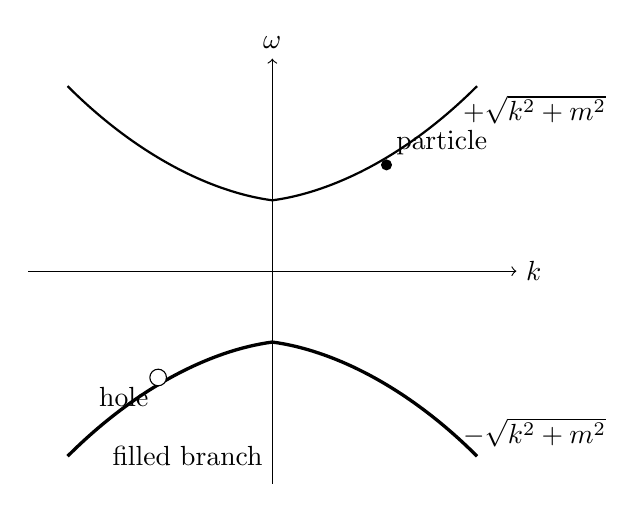
\begin{tikzpicture}[scale=1.0]
\draw[->] (-3.1,0) -- (3.1,0) node[right] {$k$};
\draw[->] (0,-2.7) -- (0,2.7) node[above] {$\omega$};
\draw[thick] (-2.6,2.35)
  .. controls (-1.7,1.45) and (-0.75,1.0) .. (0,0.9)
  .. controls (0.75,1.0) and (1.7,1.45) .. (2.6,2.35);
\draw[very thick] (-2.6,-2.35)
  .. controls (-1.7,-1.45) and (-0.75,-1.0) .. (0,-0.9)
  .. controls (0.75,-1.0) and (1.7,-1.45) .. (2.6,-2.35);
\fill (1.45,1.35) circle (2pt);
\node[above right] at (1.45,1.35) {particle};
\fill[white] (-1.45,-1.35) circle (3pt);
\draw (-1.45,-1.35) circle (3pt);
\node[below left] at (-1.45,-1.35) {hole};
\node[right] at (2.3,2.05) {$+\sqrt{k^2+m^2}$};
\node[right] at (2.3,-2.05) {$-\sqrt{k^2+m^2}$};
\node[left] at (0,-2.35) {filled branch};
\end{tikzpicture}
\caption{Bei jedem Impuls besitzt das massive Spektrum Zustände positiver und negativer Energie. Der negative Zweig ist aufgefüllt; ein fehlender Zustand darin ist ein Loch positiver Energie.}
\end{figure}
Zu jedem Impuls gibt es einen Zustand positiver und einen Zustand negativer Energie. Füllt man alle Zustände auf dem negativen Zweig auf, bleiben Teilchen positiver Energie oberhalb des Meers und Löcher positiver Energie darin zurück. Teilchen und Löcher haben beide eine positive Masse.

Der wesentliche Punkt sei noch einmal hervorgehoben. Ein Fermion wird massiv, wenn seine zwei zuvor unabhängigen Komponenten gekoppelt werden. Im Ruhezustand ist keine der ursprünglichen Komponenten für sich ein Energieeigenzustand. Die Zustände mit bestimmter Energie sind ihre Summe und ihre Differenz.

Um zu sehen, was die Summe bedeutet, bezeichnen wir die betreffenden Einteilchen-Erzeugungsanteile mit \(C_R^\dagger\) und \(C_L^\dagger\). Auf das Vakuum angewandt,
\begin{equation}
(C_R^\dagger+C_L^\dagger)\lvert0\rangle
\end{equation}
erzeugt der Ausdruck ein Teilchen in einer kohärenten Überlagerung der beiden Komponenten. Er erzeugt nicht zwei Teilchen. Ein Produkt,
\begin{equation}
C_R^\dagger C_L^\dagger\lvert0\rangle,
\end{equation}
enthält zwei Erzeugungsoperatoren und erzeugt einen Zweiteilchenzustand, sofern beide Moden verfügbar sind. Nach der Normierung hat der Ruhezustand in beiden Komponenten dieselbe Wahrscheinlichkeit; die gekoppelte Welle als Ganzes hat jedoch verschwindenden Impuls.

Die Bezeichnungen \(R\) und \(L\) kennzeichneten nur dann eine tatsächliche Bewegungsrichtung, wenn \(m=0\) galt. Sobald der Massenterm vorhanden ist, enthält eine bewegte massive Lösung im Allgemeinen beide Komponenten; die Lösung im Ruhezustand enthält sie mit gleichem Betrag. Deshalb ist es hier besser, \(R\) und \(L\) als Bezeichnungen für die obere beziehungsweise untere Spinorkomponente aufzufassen.

\begin{figure}[htbp]
\centering
\includegraphics[width=0.78\textwidth]{lecture_06_figure_04.png}
\caption{Bei von null verschiedener Masse sind die beiden Spinorkomponenten gekoppelt; die Deutung als rechts- und linkslaufend gilt unmittelbar nur im masselosen Grenzfall.}
\lectureframe{00:50:48}
\end{figure}

Alle massiven Fermionen der Teilchenphysik bestehen aus Feldern mit linken und rechten Komponenten: Eine Dirac-Masse koppelt Komponenten, die im masselosen Grenzfall unabhängig sind.

\begin{classroomqa}
\lecturetimestamp{00:52:01}
\audiencequestion{Sollte \(\psi_R\pm\psi_L\) einen Faktor \(1/\sqrt{2}\) enthalten?}
\lecturerresponse{Man kann ihn zur Normierung des Zustands einbeziehen. Er multipliziert beide Seiten der Gleichung und verändert daher die Bewegungsgleichung nicht.}
\end{classroomqa}

\begin{classroomqa}
\lecturetimestamp{00:52:12}
\audiencequestion{Spielen die relativen Beträge der rechten und linken Komponenten eine Rolle?}
\lecturerresponse{Für die gewählten Eigenzustände im Ruhesystem sind ihre Beträge gleich. Die Gesamtnormierung ist beliebig, die relativen Beträge sind jedoch durch den Eigenvektor von \(\beta\) festgelegt.}
\end{classroomqa}

\begin{classroomqa}
\lecturetimestamp{00:52:52}
\audiencequestion{Könnten die beiden Komponenten eine relative Phase haben?}
\lecturerresponse{Ja. Die reellen Koeffizienten in \(\psi_R\pm\psi_L\) ergeben sich aus der Wahl eines reellen \(\beta\). Andere Matrizen, deren Quadrat die Einheitsmatrix ist und die mit \(\alpha\) antikommutieren, sind äquivalente Wahlmöglichkeiten; dann können Phasen zwischen den Komponenten auftreten. Hat man eine Darstellung gewählt, muss man sie durchgehend verwenden.}
\end{classroomqa}

\begin{classroomqa}
\lecturetimestamp{00:53:43}
\audiencequestion{Sind die Bezeichnungen ``linkslaufend'' und ``rechtslaufend'' nach Hinzufügen der Masse irreführend?}
\lecturerresponse{In gewisser Weise. In der masselosen Theorie beschreiben sie tatsächlich linkslaufende und rechtslaufende Wellen. Bei von null verschiedener Masse enthält selbst ein Teilchen, das sich in eine bestimmte Richtung bewegt, im Allgemeinen beide Komponenten; daher sind die Bezeichnungen ``obere Komponente'' und ``untere Komponente''eindeutiger.}
\end{classroomqa}

\begin{classroomqa}
\lecturetimestamp{00:55:01}
\audiencequestion{Benötigt ein ruhendes Fermion bereits einen Eigendrehimpuls?}
\lecturerresponse{Nicht in diesem eindimensionalen Modell. In einer Raumdimension ist kein Drehimpuls definiert; der Spin ist daher noch nicht in die Konstruktion eingegangen.}
\end{classroomqa}

\begin{classroomqa}
\lecturetimestamp{00:55:24}
\audiencequestion{Enthält die Wellenfunktion fermionische Erzeugungs- und Vernichtungsoperatoren?}
\lecturerresponse{Ja.}
\end{classroomqa}

\begin{classroomqa}
\lecturetimestamp{00:55:30}
\audiencequestion{Worin zeigt sich der fermionische Charakter außer in der Wahl der Erzeugungs- und Vernichtungsoperatoren?}
\lecturerresponse{Er zeigt sich in den fermionischen Erzeugungs--- und Vernichtungsregeln. Eine Gleichung mit diesem Spektrum negativer Energien muss mit diesen Regeln quantisiert werden; bosonische Besetzungsregeln würden das Vakuum instabil lassen. Relativistische Bosonen müssen durch eine andere Wellengleichung beschrieben werden.}
\end{classroomqa}

\begin{classroomqa}
\lecturetimestamp{00:56:20}
\audiencequestion{Kann eine Lösung mit von null verschiedenem Impuls durch eine Lorentz-Transformation in die Lösung im Ruhesystem überführt werden?}
\lecturerresponse{Ja. Eine Lorentz-Transformation kann eine massive Lösung in ihr Ruhesystem überführen. Dazu muss man jedoch wissen, wie Lorentz-Transformationen auf den Spinor \(\Psi\) wirken.}
\end{classroomqa}

\section{Masse aus einem skalaren Vakuumfeld}

\begin{classroomqa}
\lecturetimestamp{00:58:11}
\audiencequestion{Wie erzeugt die Wechselwirkung mit dem Higgs-Feld den Dirac-Massenterm?}
\lecturerresponse{Man ersetzt den konstanten Massenkoeffizienten durch eine Kopplung an ein skalares Feld. Verschwindet dieses Feld im Vakuum, bleibt das Fermion masselos; besitzt es im Vakuum einen konstanten, von null verschiedenen Wert, wirkt die Kopplung genau wie eine Masse.}
\end{classroomqa}

Sei \(\phi(x,t)\) ein skalares Feld mit einer eigenen Bewegungsgleichung. In der Dirac-Gleichung ersetzen wir im Massenterm das konstante \(m\) durch \(g\phi(x,t)\):\footnote{Der dargestellte Wechselwirkungsterm entsteht, indem man diese Ersetzung im zuvor hergeleiteten Massenterm \(m\beta\Psi\) vornimmt.}
\begin{equation}
i\frac{\partial\Psi}{\partial t}
=
-i\alpha\frac{\partial\Psi}{\partial x}
+g\phi(x,t)\,\beta\Psi.
\end{equation}
Damit sind die beiden Feldgleichungen gekoppelt. Das Fermion wirkt auf das Skalarfeld ein, und das Skalarfeld wirkt auf das Fermion zurück; zusammen betrachtet ist das System nichtlinear, obwohl die Dirac-Gleichung bezüglich \(\Psi\) linear ist, wenn \(\phi\) vorgegeben ist.

Nehmen wir zunächst an, dass im leeren Raum
\begin{equation}
\phi(x,t)=0.
\end{equation}
gilt. Dann verschwindet der Mischungsterm, die obere und die untere Komponente entkoppeln sich, und das Fermion ist masselos. Nehmen wir stattdessen an, dass der Zustand niedrigster Energie ein konstantes, von null verschiedenes Skalarfeld besitzt:
\begin{equation}
\phi(x,t)=\phi_0\neq0.
\end{equation}
Dann wird die Dirac-Gleichung in diesem Vakuum zu
\begin{equation}
i\frac{\partial\Psi}{\partial t}
=
-i\alpha\frac{\partial\Psi}{\partial x}
+g\phi_0\,\beta\Psi,
\end{equation}
und damit gilt
\begin{equation}
m_{\mathrm{eff}}=g\phi_0.
\end{equation}
Eine Kopplung zwischen einem bosonischen und einem fermionischen Feld erzeugt folglich zusammen mit einem von null verschiedenen Wert des bosonischen Feldes im leeren Raum dieselbe Mischung zwischen links und rechts, die zuvor als direkt in die Gleichung eingesetzte Masse auftrat.

\begin{classroomqa}
\lecturetimestamp{01:01:27}
\audiencequestion{Könnte der LHC einen Hinweis auf ein von null verschiedenes Higgs-Feld im Vakuum liefern?}
\lecturerresponse{Unbedingt. Das ist eine der großen Fragen.}
\end{classroomqa}

\begin{classroomqa}
\lecturetimestamp{01:01:32}
\audiencequestion{Können Sie genauer erklären, wie der Higgs-Mechanismus funktioniert?}
\lecturerresponse{Ein skalares Feld besitzt Energie, die mit seinen räumlichen und zeitlichen Änderungen zusammenhängt; außerdem kann es eine lokale potenzielle Energiedichte \(V(\phi)\) geben. Liegen die Minima dieses Potenzials bei von null verschiedenen Werten von \(\phi\), enthält das Vakuum ein von null verschiedenes Feld. Quantisierte Schwingungen um das gewählte Minimum sind Higgs-Teilchen.}
\end{classroomqa}

Ein Feld kann auf zwei verschiedene Arten Energie tragen. Ein Teil der Energie hängt davon ab, wie sich das Feld räumlich und zeitlich ändert. Ein vertrautes Vergleichsbeispiel ist das Maxwell-Feld:
\begin{equation}
\mathcal{E}_{\mathrm{Maxwell}}\propto \mathbf E^2+\mathbf B^2,
\end{equation}
Sowohl \(\mathbf E\) als auch \(\mathbf B\) sind aus Ableitungen des elektromagnetischen Potenzials aufgebaut. Diese Energie ist also mit den räumlichen und zeitlichen Änderungen des zugrunde liegenden Feldes verknüpft.

Ein Skalarfeld kann außerdem eine lokale potenzielle Energiedichte besitzen,
\begin{equation}
V(\phi),
\end{equation}
die vom Wert von \(\phi\) selbst und nicht von dessen Ableitungen abhängt. Schematisch gilt
\begin{equation}
\mathcal{E}_\phi
=
\mathcal E_{\text{space and time gradients}}+V(\phi).
\end{equation}
Ohne ein tiefer liegendes Prinzip, das sie festlegt, könnte \(V(\phi)\) jede vernünftige Funktion sein, die mit den Symmetrien des Modells vereinbar ist.

Für die hier verwendete vereinfachte Veranschaulichung mit einem reellen Skalarfeld nehmen wir an, dass die Theorie unter folgender Transformation symmetrisch ist:
\begin{equation}
\phi\longrightarrow-\phi.
\end{equation}
Dann muss das Potenzial eine gerade Funktion sein:
\begin{equation}
V(\phi)=V(-\phi).
\end{equation}
Diese Symmetrie allein sagt nicht, wo das Minimum liegt. Eine Möglichkeit ist ein einziges Minimum bei \(\phi=0\). Eine andere Möglichkeit ist ein symmetrisches Paar von Minima bei von null verschiedenen Werten, einem positiven und einem negativen.

\begin{figure}[htbp]
\centering
\includegraphics[width=0.72\textwidth]{lecture_06_figure_05.png}
\caption{Ein Minimum bei \(\phi=0\) ergibt ein verschwindendes Vakuumfeld; symmetrische Minima bei von null verschiedenen Werten erlauben hingegen einen Vakuumwert \(\phi_0\neq0\) und damit eine Fermionenmasse \(g\phi_0\).}
\lectureframe{01:04:47}
\end{figure}

Die beiden Möglichkeiten lassen sich darstellen, ohne sich auf eine bestimmte Polynomform des Potenzials festzulegen.\footnote{Die folgenden Kurven zeigen nur die für das Argument nötigen qualitativen Verläufe mit einem zentrierten beziehungsweise zwei symmetrieverwandten Minima.}
\begin{figure}[htbp]
\centering
\resizebox{\linewidth}{!}{%
\begin{tikzpicture}[x=1.35cm,y=1.05cm]
\begin{scope}[shift={(-3.1,0)}]
\draw[->] (-1.7,0) -- (1.7,0) node[right] {$\phi$};
\draw[->] (0,-0.15) -- (0,2.45) node[above] {$V(\phi)$};
\draw[thick] (-1.5,2.05) .. controls (-0.9,0.65) and (-0.45,0.25) .. (0,0.25)
             .. controls (0.45,0.25) and (0.9,0.65) .. (1.5,2.05);
\fill (0,0.25) circle (1.2pt);
\node[below] at (0,0) {$0$};
\end{scope}
\begin{scope}[shift={(3.1,0)}]
\draw[->] (-1.7,0) -- (1.7,0) node[right] {$\phi$};
\draw[->] (0,-0.15) -- (0,2.45) node[above] {$V(\phi)$};
\draw[thick] (-1.55,2.05)
  .. controls (-1.25,0.75) and (-1.0,0.25) .. (-0.75,0.25)
  .. controls (-0.35,0.25) and (-0.25,1.3) .. (0,1.3)
  .. controls (0.25,1.3) and (0.35,0.25) .. (0.75,0.25)
  .. controls (1.0,0.25) and (1.25,0.75) .. (1.55,2.05);
\fill (-0.75,0.25) circle (1.2pt);
\fill (0.75,0.25) circle (1.2pt);
\node[below] at (0,0) {$0$};
\node[below] at (-0.75,0) {$-\phi_0$};
\node[below] at (0.75,0) {$\phi_0$};
\end{scope}
\end{tikzpicture}%
}
\caption{Gerade Potenziale können ein zentriertes Minimum oder zwei symmetrieverwandte Minima bei von null verschiedenen Werten haben.}
\end{figure}

Liegt das Minimum im Ursprung, gilt im Vakuum \(\phi_0=0\), und diese Kopplung verleiht dem Elektron keine Masse. Liegen die Minima bei \(\phi=\pm\phi_0\), nimmt das Vakuum einen der beiden Werte an. Die beiden Möglichkeiten sind durch die Symmetrie miteinander verknüpft, und jede von ihnen erzeugt einen von null verschiedenen Koeffizienten \(g\phi_0\) in der Dirac-Gleichung. Warum das Potenzial qualitativ diese Form hat, ist eine tiefer gehende Frage, die durch den Mechanismus selbst nicht beantwortet wird.

Das Feld muss nicht genau in seinem Minimum verharren. Es kann um den gewählten Wert schwingen, so wie ein Teilchen in der Nähe des Tiefpunkts eines Potenzialtopfs schwingen kann. Durch Quantisierung dieser Schwingungen erhält man Higgs-Quanten. Ihre charakteristische Frequenz hängt mit der Masse des Higgs-Teilchens zusammen: Bei großer Masse ist viel Energie erforderlich, um auch nur ein Quant anzuregen. Im Vakuum befindet sich das Feld einfach nahe seinem Minimum und liefert die Fermionenmasse. Schwingt das Feld, so ist diese Schwingung ein Higgs-Teilchen.

Die Kopplung bewirkt eine wechselseitige Wirkung. Fermionen reagieren auf den Wert von \(\phi\), doch ausreichend energiereiche Fermionenkollisionen können auch das Skalarfeld anregen. Eine Kollision muss die Anregungsenergie liefern; sobald das Feld schwingt, bilden seine Quanten Higgs-Teilchen. Dieses Feld koppelt nicht nur an Elektronen, sondern auch an Quarkfelder und andere Felder, deren Massen es bereitstellt.

\begin{classroomqa}
\lecturetimestamp{01:08:14}
\audiencequestion{Ändert sich die Elektronenmasse, wenn das Higgs-Feld schwingt oder ausgelenkt wird?}
\lecturerresponse{Ja. Da die effektive Masse proportional zum lokalen Feldwert ist, verringert eine Auslenkung des Feldes in Richtung null die Masse. Eine makroskopische Region weit vom Vakuumwert zu halten, würde enorme Energie erfordern; eine dafür ausreichend große Region könnte zu einem Schwarzen Loch kollabieren.}
\end{classroomqa}

Das Gedankenexperiment ist unmittelbar. Könnte man eine Region nahe \(\phi=0\) halten, so würde innerhalb dieser Region
\begin{equation}
m_{\mathrm{eff}}=g\phi
\end{equation}
klein werden oder verschwinden. Eine angeregte Higgs-Mode schwingt um den Vakuumwert, während die Erzeugung und Aufrechterhaltung einer merklichen Auslenkung über eine makroskopische Region enorme Energie erfordert. Die Kosten der potenziellen Energie wachsen mit dem Volumen. Lange bevor eine solche Region zu einem brauchbaren Labor würde, könnte ihre Energie für einen gravitativen Kollaps ausreichen. Die Massenänderung ist im Prinzip real; eine große, beobachtbare Änderung herbeizuführen ist jedoch ungeheuer schwierig.

\begin{classroomqa}
\lecturetimestamp{01:09:27}
\audiencequestion{Warum braucht man ein Higgs-Feld?}
\lecturerresponse{Weil das Elektron eine Masse hat.}
\end{classroomqa}

\begin{classroomqa}
\lecturetimestamp{01:09:41}
\audiencequestion{Hat jede Teilchenart ein eigenes Higgs-Feld?}
\lecturerresponse{Nein. Im Standardmodell liefert ein Higgs-Feld Massen für Elektronen, Quarks und die anderen Teilchen, die an diesem Mechanismus beteiligt sind. Supersymmetrische Varianten benötigen zwei Higgs-Felder statt eines separaten Feldes für jede Teilchenart.}
\end{classroomqa}

Das Bild mit einem einzigen Feld ist schematisch: Das vollständige Higgs-Feld hat eine reichere Struktur als eine einzelne reelle Zahl \(\phi\). Der wesentliche Punkt bleibt dennoch bestehen. Ein gemeinsames Vakuumfeld kann unterschiedlich stark an verschiedene Fermionen koppeln; unterschiedliche Massen erfordern daher kein eigenes Higgs-Feld für jede Teilchenart. Das Higgs-Teilchen ist eine Schwingung desselben Feldes um seinen Vakuumwert.

Warum setzt man die Elektronenmasse nicht einfach von Hand in die Gleichung ein und verzichtet auf das Higgs-Feld? Die Antwort hängt mit den schwachen Wechselwirkungen und der Vereinheitlichung zusammen; darauf kommen wir später zurück.

\begin{classroomqa}
\lecturetimestamp{01:11:16}
\audiencequestion{Gibt es in einer supersymmetrischen Theorie zwei Higgs-Sektoren?}
\lecturerresponse{Ja. In der hier verwendeten vereinfachten Einteilung liefert der eine Massen für Quarks vom Up-Typ, der andere für Quarks vom Down-Typ und für Elektronen. Diese Verdopplung ist eine technische Anforderung der Supersymmetrie, nicht die Einführung eines eigenen Higgs-Feldes für jedes Teilchen.}
\end{classroomqa}

\begin{classroomqa}
\lecturetimestamp{01:12:01}
\audiencequestion{Wenn das Higgs-Teilchen eine Masse hat, woher kommt diese Masse?}
\lecturerresponse{Diese Frage wird hier nicht beantwortet. Das präzisere Rätsel ist, warum die Higgs-Masse so klein ist.}
\end{classroomqa}

Symmetrie ist untrennbar mit der Frage der Masse verbunden. Im einfachen Dirac-Modell würde eine Symmetrie, die eine Mischung des linken und des rechten Sektors verhindert, den Koeffizienten des Mischungsterms zu null zwingen. Wenn das Vakuum diese Symmetrie respektierte, wäre das Fermion masselos. Ein von null verschiedener Higgs-Vakuumerwartungswert bricht die betreffende Vakuumsymmetrie und ermöglicht die Kopplung zwischen links und rechts:
\begin{equation}
m_{\mathrm{eff}}=g\phi_0\neq0.
\end{equation}
Die genaue Symmetrietransformation wird hier nicht ausgearbeitet; entscheidend ist ihre Auswirkung auf den Massenterm. Die Gleichungen können die Symmetrie besitzen, auch wenn der konkrete Zustand niedrigster Energie sie nicht besitzt. Diese Asymmetrie des Vakuums liefert die Masse.

Im hier skizzierten elektroschwachen Bild erhalten Elektronen und Quarks auf diese Weise Masse, ebenso die Bosonen \(W\) und \(Z\). Das Photon bleibt masselos. Das Higgs-Teilchen selbst ist eine weitere Ausnahme: Es kann auch ohne dieselbe Verschiebung des Vakuums Masse haben; seine Masse betrifft Schwingungen seines eigenen Feldes und nicht die Mischung linker und rechter Fermionen. In dieser Darstellung erzeugt der Higgs-Vakuumerwartungswert also die Massen der übrigen Teilchen, während die Masse der Higgs-Anregung eine gesonderte Frage aufwirft.

\begin{classroomqa}
\lecturetimestamp{01:15:26}
\audiencequestion{Hat das Graviton Masse?}
\lecturerresponse{Nein. Das Graviton ist wie das Photon masselos. Früher nahm man auch an, Neutrinos seien masselos; tatsächlich haben sie jedoch eine sehr kleine Masse. In der hier verwendeten Sprache bedeutet das, dass ihre linken und rechten Komponenten nur sehr schwach gekoppelt sind.}
\end{classroomqa}

Photonen und der Theorie zufolge auch Gravitonen sind masselos und bewegen sich mit Lichtgeschwindigkeit. Neutrinos gehören nicht ganz zu dieser Klasse. Ihre winzige Masse bedeutet in dieser Dirac-Sprache, dass die Kopplung zwischen ihren linken und rechten Komponenten winzig ist. Warum sie so klein ist, ist eine andere Frage.

\section{Die Dirac-Gleichung in drei Raumdimensionen}

In drei Raumdimensionen wird die Wellenzahl zu einem Wellenvektor,
\begin{equation}
\mathbf{k}=(k_1,k_2,k_3),
\end{equation}
mit Komponenten in den Richtungen \(x\), \(y\) und \(z\). Die eindimensionale Beziehung lautet
\begin{equation}
\omega=\alpha k+\beta m,
\end{equation}
und ihre einfachste lineare Verallgemeinerung ist
\begin{equation}
\omega
=
\alpha_1 k_1+\alpha_2 k_2+\alpha_3 k_3+\beta m.
\end{equation}
Hier sind \(\alpha_i\) und \(\beta\) Matrizen. Sie müssen so gewählt werden, dass
\begin{equation}
\omega^2=k_1^2+k_2^2+k_3^2+m^2.
\end{equation}
Diese invariante Dispersionsrelation ist eine wesentliche Bedingung, für sich genommen aber nicht der gesamte Inhalt der Relativitätstheorie.

Quadriert man den linearen Ausdruck, erhält man
\begin{align}
\omega^2
={}&
\alpha_1^2k_1^2+\alpha_2^2k_2^2+\alpha_3^2k_3^2+\beta^2m^2
\nonumber\\
&+(\alpha_1\alpha_2+\alpha_2\alpha_1)k_1k_2
+(\alpha_1\alpha_3+\alpha_3\alpha_1)k_1k_3
\nonumber\\
&+(\alpha_2\alpha_3+\alpha_3\alpha_2)k_2k_3
+\sum_{i=1}^{3}(\alpha_i\beta+\beta\alpha_i)k_i m.
\end{align}
Die Koeffizienten der quadrierten Impulse und der Masse müssen erfüllen:
\begin{equation}
\alpha_1^2=\alpha_2^2=\alpha_3^2=I,
\qquad
\beta^2=I.
\end{equation}
Die unerwünschten Terme \(k_i k_j\) verschwinden, wenn verschiedene Matrizen \(\alpha\) antikommutieren:
\begin{equation}
\alpha_i\alpha_j+\alpha_j\alpha_i=0,
\qquad i\neq j.
\end{equation}
Die gemischten Terme \(k_i m\) verschwinden, wenn
\begin{equation}
\alpha_i\beta+\beta\alpha_i=0
\qquad
\text{for each }i.
\end{equation}
Damit quadrieren alle vier Matrizen zur Einheitsmatrix, und jedes Paar verschiedener Matrizen antikommutiert.

Drei Matrizen \(2\times2\) mit den erforderlichen paarweisen Antikommutationseigenschaften gibt es: Es sind die drei Pauli-Matrizen. Es gibt keine vierte Matrix \(2\times2\), die sowohl zur Einheitsmatrix quadriert als auch mit allen dreien antikommutiert. Auch keine Realisierung mit Matrizen \(3\times3\) ist möglich. Die kleinste mögliche Realisierung verwendet Matrizen \(4\times4\), die Dirac-Matrizen.

Der Übergang von zwei zu vier Komponenten wirft eine physikalische Frage auf. In einer Raumdimension begannen die beiden Komponenten als rechts- und linkslaufende Felder. Was bedeuten vier Komponenten? Der neue Bestandteil ist der Spin, doch für den Spin braucht man den Drehimpuls und damit eine echte dreidimensionale Betrachtung.

Die Matrizen sind nicht eindeutig. Verschiedene Wahlmöglichkeiten sind in etwa so gleichwertig wie verschiedene Wahlen paarweise orthogonaler Koordinatenachsen: Die Einträge ändern sich, aber eine Transformation verknüpft die Beschreibungen, und die Physik bleibt unverändert. Eine zweckmäßige Darstellung ist\footnote{Die folgenden Matrizen in Eintragsform sind die ausgeschriebene Form der Blockdarstellung und der Pauli-Matrizen, die unmittelbar danach angegeben werden; diese Blockbeziehungen werden in der Vorlesung bei 01:30:23--01:31:29 ausdrücklich angegeben.}
\begin{equation}
\beta=
\begin{pmatrix}
1&0&0&0\\
0&1&0&0\\
0&0&-1&0\\
0&0&0&-1
\end{pmatrix},
\end{equation}
zusammen mit
\begin{align}
\alpha_1&=
\begin{pmatrix}
0&0&0&1\\
0&0&1&0\\
0&1&0&0\\
1&0&0&0
\end{pmatrix},
&
\alpha_2&=
\begin{pmatrix}
0&0&0&-i\\
0&0&i&0\\
0&-i&0&0\\
i&0&0&0
\end{pmatrix},
\\[1ex]
\alpha_3&=
\begin{pmatrix}
0&0&1&0\\
0&0&0&-1\\
1&0&0&0\\
0&-1&0&0
\end{pmatrix}.
\end{align}
Ihre Struktur lässt sich leichter erkennen, wenn man jede Matrix in Blöcke \(2\times2\) unterteilt:
\begin{equation}
\beta=
\begin{pmatrix}
I_2&0\\
0&-I_2
\end{pmatrix},
\qquad
\alpha_i=
\begin{pmatrix}
0&\sigma_i\\
\sigma_i&0
\end{pmatrix}.
\end{equation}
Die drei Pauli-Matrizen sind
\begin{equation}
\sigma_1=
\begin{pmatrix}
0&1\\
1&0
\end{pmatrix},
\quad
\sigma_2=
\begin{pmatrix}
0&-i\\
i&0
\end{pmatrix},
\quad
\sigma_3=
\begin{pmatrix}
1&0\\
0&-1
\end{pmatrix}.
\end{equation}
Diese Blockmatrizen erfüllen die erforderlichen Antikommutationsrelationen der Dirac-Matrizen.

Die Wellenfunktion muss nun vier Komponenten haben:
\begin{equation}
\Psi=
\begin{pmatrix}
\psi_1\\
\psi_2\\
\psi_3\\
\psi_4
\end{pmatrix}.
\end{equation}
Die Bewegungsgleichung lautet
\begin{equation}
i\frac{\partial\Psi}{\partial t}
=
-i\sum_{j=1}^{3}\alpha_j
\frac{\partial\Psi}{\partial x_j}
+\beta m\Psi.
\end{equation}
Dieser kompakte Ausdruck steht für vier gekoppelte lineare Differentialgleichungen. Die Nebendiagonaleinträge der \(\alpha_j\) koppeln die vier Komponenten auf komplexere Weise als im eindimensionalen Fall, doch die Grundstruktur ist dieselbe: Matrizen koppeln die Komponenten, während die Gleichung in Raum und Zeit erster Ordnung bleibt. Die zusätzliche Verdopplung der Komponenten ist der Hinweis, der zum Spin führt.

\begin{classroomqa}
\lecturetimestamp{01:33:53}
\audiencequestion{Sind die vier Komponenten von \(\Psi\) ein Vierervektor, der direkt den vier Dimensionen der Raumzeit zugeordnet ist?}
\lecturerresponse{Nein. Sie bilden einen Spinor, keinen Vierervektor. Die Übereinstimmung zwischen den zwei Raumzeitdimensionen und den zwei Spinorkomponenten im eindimensionalen Beispiel war zufällig. In höherdimensionalen Konstruktionen treten Spinormatrizen mit Größen auf, die Zweierpotenzen sind und im Allgemeinen nicht der Anzahl der Raumzeitdimensionen entsprechen.}
\end{classroomqa}

Auch hier liefert das Ruhesystem die einfachste Interpretation. Bei verschwindendem Impuls verschwindet der Ableitungsterm:
\begin{equation}
i\frac{\partial\Psi}{\partial t}=m\beta\Psi.
\end{equation}
In der gewählten Darstellung hat \(\beta\) zwei Eigenwerte \(+1\) und zwei Eigenwerte \(-1\). Es gibt daher zwei Ruhezustände mit der Energie \(+m\) und zwei mit der Energie \(-m\). Wie zuvor sind die Zustände negativer Energie aufgefüllt. Die zweifache Entartung bei jedem Energievorzeichen ist die zusätzliche Struktur, deren physikalische Interpretation der Spin ist.

\begin{classroomqa}
\lecturetimestamp{01:35:51}
\audiencequestion{Sollten die Nebendiagonalblöcke in \(\alpha_i\) denselben Index tragen, sodass sie \(\sigma_i\) sind?}
\lecturerresponse{Ja. Jede Matrix \(\alpha_i\) enthält die entsprechende Pauli-Matrix \(\sigma_i\) in beiden Nebendiagonalblöcken.}
\end{classroomqa}

\begin{classroomqa}
\lecturetimestamp{01:36:03}
\audiencequestion{Fehlt in der kompakten Antikommutationsrelation für die \(\alpha_i\) ein Faktor zwei?}
\lecturerresponse{Ja. Für \(i=j\) ist die linke Seite gleich \(\alpha_i^2+\alpha_i^2=2I\). Die korrekte Relation lautet \(\alpha_i\alpha_j+\alpha_j\alpha_i=2\delta_{ij}I\).}
\end{classroomqa}

Die Bedingungen für gleiche und verschiedene Indizes lassen sich daher zusammenfassen zu
\begin{equation}
\alpha_i\alpha_j+\alpha_j\alpha_i=2\delta_{ij}I.
\end{equation}

\begin{classroomqa}
\lecturetimestamp{01:36:42}
\audiencequestion{War der Übergang zu vier Matrizen in Diracs Konstruktion ein großer konzeptioneller Schritt?}
\lecturerresponse{Ja. Dirac postulierte die Gleichung und verfolgte ihre Konsequenzen. Eine davon war das Auftreten von Antiteilchen, eine andere der Spin. Der Spin war bereits empirisch bekannt, aber die Gleichung erklärte ihn.}
\end{classroomqa}

\begin{classroomqa}
\lecturetimestamp{01:37:29}
\audiencequestion{Was kam zuerst: der empirische Nachweis oder der Satz, der Teilchen auf Bosonen und Fermionen beschränkt?}
\lecturerresponse{Der empirische Nachweis kam zuerst, der Satz später. Die Alternative Boson--Fermion gilt in drei Raumdimensionen. In zwei Raumdimensionen mit einer Zeitdimension kann es Zwischenstatistiken geben; in \(3+1\) Dimensionen und in höheren Raumdimensionen gibt es die Alternative zwischen Bosonen und Fermionen.}
\end{classroomqa}

\begin{classroomqa}
\lecturetimestamp{01:39:01}
\audiencequestion{Gibt es eine übliche Indexbezeichnung für die vier Komponenten von \(\Psi\)?}
\lecturerresponse{Hier ist keine bestimmte Wahl wesentlich. Man kann die Bezeichnungen \(p\) und \(q\) verwenden, die von eins bis vier laufen; dann hat jede Matrix einen Zeilenindex und einen Spaltenindex.}
\end{classroomqa}

Die Matrixnotation lässt diese Komponentenindizes weg. Schreibt man sie explizit hin, gilt
\begin{equation}
p,q=1,2,3,4,
\end{equation}
und die Gleichung lautet
\begin{equation}
i\,\partial_t\Psi_p
=
-i\sum_{j=1}^{3}\sum_{q=1}^{4}
(\alpha_j)_{pq}\,\partial_j\Psi_q
+m\sum_{q=1}^{4}\beta_{pq}\Psi_q.
\end{equation}

\begin{classroomqa}
\lecturetimestamp{01:40:15}
\audiencequestion{Sind die expliziten Komponentenindizes überflüssig, wenn man Matrixmultiplikation verwendet?}
\lecturerresponse{Ja. Die Matrixnotation lässt diese Indizes automatisch weg. Eine symmetrischere Form, die die relativistische Struktur deutlicher macht, kann später eingeführt werden.}
\end{classroomqa}

Die dargestellte Gleichung ist die Dirac-Gleichung in ihrer einfachsten Form in \(3+1\) Dimensionen. Als Nächstes geht es darum, den Spin zu verstehen und Wellengleichungen für relativistische Bosonen aufzustellen, denn die Dirac-Gleichung ist nicht ihre Gleichung, und etwa die Hälfte der Teilchen in der Natur sind Bosonen. Mit diesen Bausteinen kann man sich Quarks, Leptonen, schwachen Bosonen, Higgs-Teilchen und Photonen zuwenden und Ordnung in das Teilchenspektrum bringen. Für die gesamte Diskussion wird mehr Symmetrie benötigt.
